\documentclass[xcolor=table,dvipsnames,table]{beamer}
\mode<presentation>
\usetheme{boxes}
\setbeamertemplate{navigation symbols}{}
% http://www.latex-community.org/forum/viewtopic.php?f=4&t=6694
\setbeamertemplate{navigation symbols}{\raisebox{5pt}{\makebox[\paperwidth]{\hfill\makebox[10pt]{\scriptsize\insertframenumber\vspace{1ex}}}}}
%\setbeamertemplate{footline}[frame number]
\setbeamertemplate{blocks}[shadow=false]
%\setbeamercolor*{block title}{fg=structure,bg=RoyalBlue!10}
\setbeamercolor*{block title example}{fg=structure,bg=RoyalBlue!10}
%\setbeamercolor*{block title example}{fg=BrickRed,bg=Goldenrod!10}
\setbeamercolor*{block title alerted}{fg=white,bg=black}
\addtobeamertemplate{block begin}{\pgfsetfillopacity{0.8}}{\pgfsetfillopacity{1}}
%\rowcolors{0}{RoyalBlue!20}{RoyalBlue!5}
\setbeamertemplate{caption}{\raggedright\insertcaption\par}

%\DeclareGraphicsRule{*}{mps}{*}{}

\usepackage{latexsym}
\usepackage{hyperref}
\usepackage{tikz}
\usetikzlibrary{calc,shapes,arrows,shadows,shapes.callouts,shapes.arrows,chains,positioning,trees}
\usepackage{solution}
\usepackage{calc}
\usepackage{pifont}
\usepackage{algorithmic}
\usepackage{pdfcomment}
\usepackage{color}

\newcommand{\cmark}{\ding{51}}
\newcommand{\xmark}{\ding{55}}

\newcommand{\highlight}[1]{{\color{blue}{#1}}}
\newcommand{\mycite}[1]{{\color{darkgray}{\footnotesize [#1]}}}

\DeclareMathOperator*{\argmin}{arg\,min}
\DeclareMathOperator*{\argmax}{arg\,max}
\DeclareMathOperator{\sign}{sign}
\DeclareMathOperator{\cnt}{Count}

\newcounter{mycallout}

\newcommand{\callouts}[3]{%
  \stepcounter{mycallout}
  \tikz[remember picture,baseline]{\node[anchor=base,inner sep=0,outer sep=0]%
    (\themycallout) {\colorbox{#1!20}{#3}};\pause\node[overlay,rectangle callout,%
    callout relative pointer={(0cm,0.5cm)},fill=#1!20] at ($(\themycallout.south)+(-0cm,-0.7cm)$){#2};}%
    }%

\raggedright

\newcount\lecturecount
\lecturecount=0
\AtBeginLecture{%
    \advance\lecturecount by 1
    \date{}
    \begin{frame}
    \begin{center}
    \titlepage
    \ifnum\lecturecount=1
    Part \the\lecturecount: \insertlecture
    \else
    Part \the\lecturecount: \insertlecture
    \fi
    \end{center}
    \end{frame}
}

\addtobeamertemplate{block begin}{\setlength\abovedisplayskip{0pt}}

%\newcommand{\example}[1]{{\color{BrickRed!50}{#1}}}
\newcommand{\maths}[1]{{\color{RoyalBlue!50}{#1}}}
\newcommand{\reference}[1]{{\color{RoyalBlue!30}\tiny [from #1]}}
\newcommand{\koehnref}{\reference{\href{http://www.statmt.org/book}{P.Koehn SMT book slides}}}


\begin{document}

\title{\color{MidnightBlue}Natural Language Processing}

\author{Anoop Sarkar \\ {\color{RoyalBlue!70}{\href{http://anoopsarkar.github.io/nlp-class}{anoopsarkar.github.io/nlp-class}}}}
\institute{\color{BrickRed}Simon Fraser University}
%\date{}
     
{
\addtocounter{framenumber}{-1}
\begin{frame}
\begin{center}
\vspace{8mm}

\includegraphics[scale=0.35]{figures/natlang-cky-logo}
\end{center}
\titlepage
\end{frame}
}



\lecture{Probability models of Language}{}
\section{Language models}

\begin{frame}
\frametitle{The Language Modeling problem}
\begin{block}{Setup}
\begin{itemize}[<+->]
\item Assume a (finite) vocabulary of words:
\[ {\cal V} = \{ killer, crazy, clown \} \]
\item Use ${\cal V}$ to construct an infinite set of \textit{sentences} 
\begin{eqnarray*} 
{\cal V}^+ = & \{ & \\
&& \mbox{clown, killer clown, crazy clown, } \\
&& \mbox{crazy killer clown, killer crazy clown}, \\
&& \ldots \\
& \} &
\end{eqnarray*}
\item A \textit{sentence} is \textbf{defined} as each $s \in {\cal V}^+$
\end{itemize}
\end{block}
\end{frame}

\begin{frame}
\frametitle{The Language Modeling problem}
\begin{block}{Data}
Given a training data set of example sentences $s \in {\cal V}^+$
\end{block}
\pause
\begin{columns}
\column{0.5\linewidth}
    \begin{block}{Language Modeling problem}
    Estimate a probability model:
    \[ \sum_{s \in {\cal V}^+} p(s) = 1.0 \]
    \end{block}
\column{0.5\linewidth}
    \begin{block}{}
    \begin{itemize}
    \item p(clown) = 1e-5
    \item p(killer) = 1e-6
    \item {\small p(killer clown) = 1e-12}
    \item {\footnotesize p(crazy killer clown) = 1e-21}
    \item {\tiny p(crazy killer clown killer) = 1e-110}
    \item {\tiny p(crazy clown killer killer) = 1e-127}
    \end{itemize}
    \end{block}
\end{columns}
\begin{alertblock}{Why do we want to do this?}
\end{alertblock}
\end{frame}

\begin{frame}
\frametitle{Scoring Hypotheses in Speech Recognition}
\centering
\begin{block}{From acoustic signal to candidate transcriptions}
\begin{tabular}{ll}
\rowcolor{MidnightBlue!50}
Hypothesis & Score \\
\hline
the station signs are in deep in english & -14732 \\
the stations signs are in deep in english & -14735 \\
the station signs are in deep into english & -14739 \\
the station 's signs are in deep in english & -14740 \\
the station signs are in deep in the english & -14741 \\
the station signs are indeed in english & -14757 \\
the station 's signs are indeed in english & -14760 \\ 
the station signs are indians in english & -14790 \\
the station signs are indian in english & -14799 \\
the stations signs are indians in english & -14807 \\
the stations signs are indians and english & -14815 
\end{tabular}
\end{block}
\end{frame}

\begin{frame}[fragile]
\frametitle{Scoring Hypotheses in Machine Translation}
\centering
\begin{block}{From source language to target language candidates}
\begin{tabular}{ll}
\rowcolor{MidnightBlue!50}
Hypothesis & Score \\
\hline
we must also discuss a vision . & -29.63 \\
we must also discuss on a vision . & -31.58 \\
it is also discuss a vision . & -31.96 \\
we must discuss on greater vision . & -36.09 \\
\vdots & \vdots \\
\end{tabular}
\end{block}
\end{frame}

\begin{frame}
\frametitle{Scoring Hypotheses in Decryption}
\centering
\begin{block}{Character substitutions on ciphertext to plaintext candidates}
\begin{tabular}{ll}
\rowcolor{MidnightBlue!50}
Hypothesis & Score \\
\hline
Heopaj, zk ukq swjp pk gjks w oaynap? & -93\\
Urbcnw, mx hxd fjwc cx twxf j bnlanc? & -92\\
Wtdepy, oz jzf hlye ez vyzh l dpncpe? & -91\\
Mjtufo, ep zpv xbou up lopx b tfdsfu? & -89\\
Nkuvgp, fq aqw ycpv vq mpqy c ugetgv? & -87\\
Gdnozi, yj tjp rvio oj fijr v nzxmzo? & -86\\
Czjkve, uf pfl nrek kf befn r jvtivk? & -85\\
Yvfgra, qb lbh jnag gb xabj n frperg? & -84\\
Zwghsb, rc mci kobh hc ybck o gsqfsh? & -83\\
Byijud, te oek mqdj je adem q iushuj? & -77\\
Jgqrcl, bm wms uylr rm ilmu y qcapcr? & -76\\
Listen, do you want to know a secret? & -25\\
\end{tabular}
\end{block}
\end{frame}

\begin{frame}
\frametitle{Scoring Hypotheses in Spelling Correction}
\centering
\begin{block}{Substitute spelling variants to generate hypotheses}
\begin{tabular}{p{8cm}l}
\rowcolor{MidnightBlue!50}
Hypothesis & Score \\
\hline
... stellar and versatile {\color{MidnightBlue}\textbf{acress}} whose combination of sass and glamour has defined her ... & -18920 \\
... stellar and versatile {\color{MidnightBlue}\textbf{acres}} whose combination of sass and glamour has defined her ... & -10209 \\
... stellar and versatile {\color{MidnightBlue}\textbf{actress}} whose combination of sass and glamour has defined her ... & -9801
\end{tabular}
\end{block}
\end{frame}

\begin{frame}
\frametitle{T9 to English}
\framesubtitle{Grover, King, \& Kushler. 1998. \\Reduced keyboard disambiguating computer. US Patent 5,818,437}
\begin{columns}
\begin{column}{0.25\textwidth}
\centering
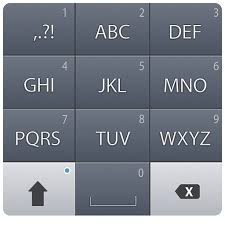
\includegraphics[scale=.4]{figures/android_t9.jpg}
\end{column}
\begin{column}{0.75\textwidth}  %%<--- here
\begin{block}{Sequence of numbers to English}
\begin{tabular}{p{3cm}p{3cm}l}
\rowcolor{MidnightBlue!50}
Input & Hypothesis & Score \\
\hline
46 04663 & GO HOOD & -24 \\
46 04663 & GO HOME & -10 \\
843 0746453 06678 07678527 0243373 0460843 096753 & ? & ? \end{tabular} % THE SINGLE MOST POPULAR CHEESE IN THE WORLD
\end{block}
\end{column}
\end{columns}

\end{frame}

\begin{frame}
\frametitle{Probability models of language}
\centering
\begin{alertblock}{Question}
\begin{itemize}[<+->]
\item Given a finite vocabulary set ${\cal V}$
\item We want to build a probability model $P(s)$ for all $s \in {\cal V}^+$
\item \textbf{But} we want to consider sentences $s$ of each length $\ell$ separately.
\item Write down a new model over ${\cal V}^+$ such that $P(s \mid \ell)$ is in the model 
\item \textbf{And} the model should be equal to $\sum_{s \in {\cal V}^+} P(s)$.
\item Write down the model
\[ \sum_{s \in {\cal V}^+} P(s) = \ldots \]
\end{itemize}
\end{alertblock}
\end{frame}

\lecture{$n$-grams for Language Modeling}{}
\section{$n$-grams for Language Modeling}
\frame{\tableofcontents[currentsection]}

\begin{frame}
\frametitle{$n$-gram Models}
\centering
\begin{block}{Google $n$-gram viewer}
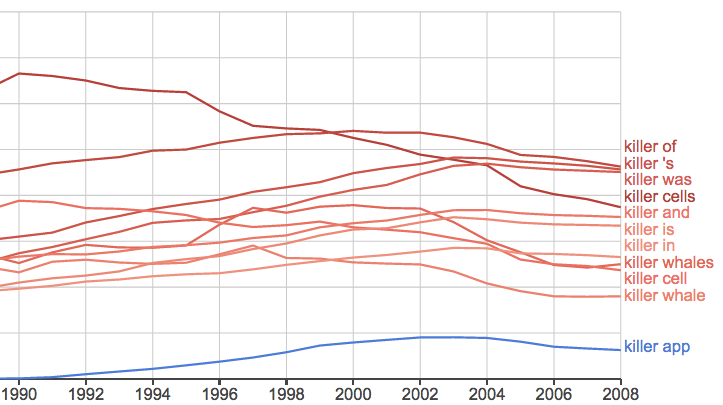
\includegraphics[scale=0.45]{figures/killer-ngrams.png}
\end{block}
\end{frame}

\begin{frame}
\frametitle{Learning Language Models}
\begin{itemize}[<+->]
\item Directly count using a training data set of sentences: $w_1, \ldots, w_n$:
\[ p(w_1, \ldots, w_n) = \frac{c(w_1, \ldots, w_n)}{N} \]
\item $c$ is a function that counts how many times each sentence occurs
\item $N$ is the sum over all possible $c(\cdot)$ values
\item Problem: does not generalize to new sentences unseen in the training data.
\item What are the chances you will see a sentence: \texttt{crazy killer clown crazy killer}?
\item In NLP applications we often need to assign non-zero probability to previously unseen sentences.
\end{itemize}
\end{frame}

\begin{frame}
\frametitle{Learning Language Models}
\begin{block}{Apply the Chain Rule: the unigram model}
\begin{eqnarray*}
p(w_1, \ldots, w_n) &\approx& p(w_1) p(w_2) \ldots p(w_n) \\
&=& \prod_i p(w_i)
\end{eqnarray*}
\end{block}
\pause
\begin{block}{Big problem with a unigram language model}
\[ p(\textsf{the the the the the the the}) > p(\textsf{we must also discuss a vision .}) \]
\end{block}

\end{frame}


\begin{frame}
\frametitle{Learning Language Models}
\begin{block}{Apply the Chain Rule: the bigram model}
\begin{eqnarray*}
p(w_1, \ldots, w_n) &\approx& p(w_1) p(w_2 \mid w_1) \ldots p(w_n \mid w_{n-1}) \\
&=& p(w_1) \prod_{i=2}^n p(w_i \mid w_{i-1})
\end{eqnarray*}
\end{block}
\pause
\begin{block}{Better than unigram}
\[ p(\textsf{the the the the the the the}) < p(\textsf{we must also discuss a vision .}) \]
\end{block}
\end{frame}

\begin{frame}
\frametitle{Learning Language Models}
\begin{block}{Apply the Chain Rule: the trigram model}
\begin{eqnarray*}
\lefteqn{p(w_1, \ldots, w_n) \approx} \\
&& p(w_1) p(w_2 \mid w_1) p(w_3 \mid w_1, w_2) \ldots p(w_n \mid w_{n-2}, w_{n-1}) \\
&& p(w_1) p(w_2 \mid w_1) \prod_{i=3}^n p(w_i \mid w_{i-2}, w_{i-1})
\end{eqnarray*}
\end{block}
\pause
\begin{block}{Better than bigram, but $\ldots$}
p(\textsf{we must also discuss a vision .}) might be zero because we have not seen p(discuss $\mid$ must also)
\end{block}
\end{frame}

\begin{frame}
\frametitle{Maximum Likelihood Estimate}
\begin{block}{Using training data to learn a trigram model}
\begin{itemize}[<+->]
\item Let $c(u,v,w)$ be the count of the trigram $u,v,w$, e.g. $c(crazy,killer,clown)$. $P(u,v,w) = \frac{c(u,v,w)}{\sum_{u,v,w} c(u,v,w)}$
\item Let $c(u,v)$ be the count of the bigram $u,v$, e.g. $c(crazy,killer)$. $P(u,v) = \frac{c(u,v)}{\sum_{u,v} c(u,v)}$
\item For any $u,v,w$ we can compute the conditional probability of generating $w$ given $u,v$:
\[ p(w \mid u,v) = \frac{c(u,v,w)}{c(u,v)} \]
\item For example:
\[ p(clown \mid crazy, killer) = \frac{c(crazy, killer, clown)}{c(crazy, killer)} \]
\end{itemize}

\end{block}
\end{frame}

\begin{frame}
\frametitle{Number of Parameters}
\begin{block}{How many probabilities in each $n$-gram model}
\begin{itemize}
\item Assume ${\cal V} = \{ \textit{killer}, \textit{crazy}, \textit{clown}, \textit{UNK} \}$
\end{itemize}
\end{block}
\pause
\begin{alertblock}{Question}
\callouts{blue}{4}{How many unigram probabilities: $P(x)$ for $x \in {\cal V}$?}
\end{alertblock}
\end{frame}

\begin{frame}
\frametitle{Number of Parameters}
\begin{block}{How many probabilities in each $n$-gram model}
\begin{itemize}
\item Assume ${\cal V} = \{ \textit{killer}, \textit{crazy}, \textit{clown}, \textit{UNK} \}$
\end{itemize}
\end{block}
\pause
\begin{alertblock}{Question}
\callouts{blue}{$4^2=16$}{How many bigram probabilities: $P(y|x)$ for $x,y \in {\cal V}$?}
\end{alertblock}
\end{frame}

\begin{frame}
\frametitle{Number of Parameters}
\begin{block}{How many probabilities in each $n$-gram model}
\begin{itemize}
\item Assume ${\cal V} = \{ \textit{killer}, \textit{crazy}, \textit{clown}, \textit{UNK} \}$
\end{itemize}
\end{block}
\pause
\begin{alertblock}{Question}
\callouts{blue}{$4^3=64$}{How many trigram probabilities: $P(z|x,y)$ for $x,y,z \in {\cal V}$?}
\end{alertblock}
\end{frame}

\begin{frame}
\frametitle{Number of Parameters}
\begin{alertblock}{Question}
\begin{itemize}
\item Assume $\mid {\cal V} \mid$ = 50,000 (a realistic vocabulary size for English)
\item What is the minimum size of training data in tokens?
\begin{itemize}
\item If you wanted to observe all unigrams at least once.
\item \callouts{blue}{125,000,000,000,000 (125 Ttokens)}{If you wanted to observe all trigrams at least once.}
\end{itemize}
\end{itemize}
\end{alertblock}
\bigskip
\begin{block}{}
Some trigrams should be zero since they do not occur in the language, $P(the \mid the, the)$. \\
But others are simply unobserved in the training data, $P(idea \mid colourless, green)$.
\end{block}
\end{frame}

\subsection{Handling Unknown Tokens}

\begin{frame}
\frametitle{Handling tokens in test corpus unseen in training corpus}
\begin{block}{Assume closed vocabulary}
In some situations we can make this assumption, e.g.\ our vocabulary is ASCII characters
\end{block}
\pause
\begin{block}{Interpolate with unknown words distribution}
We will call this {\em smoothing}. We combine the $n$-gram probability with a distribution over unknown words 
\smallskip
\[ P_{\textrm{unk}}(w) = \frac{1}{V_{\textrm{all}}} \] 
$V_{\textrm{all}}$ is an estimate of the vocabulary size including unknown words.
\end{block}
\pause
\begin{block}{Add an \texttt{<unk>} word}
Modify the training data $L$ by changing words that appear only once to the \texttt{<unk>} token. Since this probability can be an over-estimate we multiply it with a probability $P_{\textrm{unk}}(\cdot)$.
\end{block}

\end{frame}

\lecture{Smoothing Probability Models}{}
\section{Smoothing $n$-gram Models}
\frame{\tableofcontents[currentsection]}

\begin{comment}

\subsection{Smoothing Counts}

\begin{frame}
\frametitle{Bigram Models}
\begin{itemize}[<+->]
\item
In practice: 
\begin{eqnarray*}
\lefteqn{P(\texttt{crazy killer clown})=}\\
&& P(\texttt{crazy}~\mid~\texttt{<s>}) \times P(\texttt{killer}~\mid~\texttt{crazy}) \times \\
&& P(\texttt{clown}~\mid~\texttt{killer}) \times P(\texttt{</s>}~\mid~\texttt{clown})
\end{eqnarray*}

\item $P(w_i~\mid~w_{i-1}) = \frac{ c(w_{i-1},w_i) } { c(w_{i-1}) }$ \\
 On unseen data, $c(w_{i-1},w_i)$ or worse $c(w_{i-1})$ could be zero
\[ \sum_{w_i} \frac{ c(w_{i-1},w_i) } { c(w_{i-1}) } = ? \]

\end{itemize}
\end{frame}


\begin{frame}
\frametitle{Smoothing}
\begin{itemize}[<+->]

\item {\bf Smoothing} deals with events that have been observed zero times

\item Smoothing algorithms also tend to improve the accuracy of the model

\[ P(w_i~\mid~w_{i-1}) = \frac{ c(w_{i-1},w_i) } { c(w_{i-1}) } \]

\item Not just unobserved events: what about events observed once?
\end{itemize}
\end{frame}

\subsubsection{Add-one Smoothing}

\begin{frame}
\frametitle{Add-one Smoothing}
\[ P(w_i~\mid~w_{i-1}) = \frac{ c(w_{i-1},w_i) } { c(w_{i-1}) } \]
\begin{itemize}[<+->]
\item Add-one Smoothing:
\[ P(w_i~\mid~w_{i-1}) = \frac{ 1 + c(w_{i-1},w_i) } { V + c(w_{i-1}) } \]
\item Let $V$ be the number of words in our vocabulary \\
 Assign count of $1$ to unseen bigrams
\end{itemize}
\end{frame}

\begin{frame}
\frametitle{Add-one Smoothing}
\begin{eqnarray*}
\lefteqn{P(\texttt{insane killer clown})=}\\
&& P(\texttt{insane}~\mid~\texttt{<s>}) \times P(\texttt{killer}~\mid~\texttt{insane}) \times \\
&& P(\texttt{clown}~\mid~\texttt{killer}) \times P(\texttt{</s>}~\mid~\texttt{clown})
\end{eqnarray*}
\begin{itemize}[<+->]
\item Without smoothing:
\[ P(\texttt{killer}~\mid~\texttt{insane}) = \frac{ c(\texttt{insane, killer}) } { c(\texttt{insane}) }  = 0 \]
\item With add-one smoothing (assuming initially that \texttt{c(insane)} = 1 and \texttt{c(insane, killer)} = 0):
\[ P(\texttt{killer}~\mid~\texttt{insane}) = \frac{ 1 } { V + 1 }  \]
\end{itemize}
\end{frame}

\subsubsection{Additive Smoothing}

\begin{frame}
\frametitle{Additive Smoothing: (Lidstone 1920, Jeffreys 1948)} 
\[ P(w_i~\mid~w_{i-1}) = \frac{ c(w_{i-1},w_i) } { c(w_{i-1}) } \]
\begin{itemize}[<+->]
\item Why add $1$? $1$ is an overestimate for unobserved events.
\item Additive Smoothing:
\[ P(w_i~\mid~w_{i-1}) = \frac{ \delta + c(w_{i-1},w_i) } { (\delta \times V) + c(w_{i-1}) } \]
\item $0 < \delta \leq 1$
\end{itemize}
\end{frame}

\subsubsection{Good-Turing Smoothing}

\begin{frame}
\frametitle{Good-Turing Smoothing: (Good, 1953)} 
\[ P(w_i~\mid~w_{i-1}) = \frac{ c(w_{i-1},w_i) } { c(w_{i-1}) } \]
\begin{itemize}[<+->]
\item Imagine you're sitting at a sushi bar with a conveyor belt. 
\item You see going past you  { \color{blue} 10} plates of tuna,  { \color{blue} 3} plates of unagi,  { \color{blue} 2} plates of salmon,  { \color{blue} 1} plate of shrimp,  { \color{blue} 1} plate of octopus, and  { \color{blue} 1} plate of yellowtail
\item Chance you will observe a \alert{new} kind of seafood: {\color{blue} $\frac{3}{18}$}
\item How likely are you to see another plate of salmon: \\
should be { \color{blue} $< \frac{2}{18}$ }
\end{itemize}
\end{frame}

\begin{frame}
\frametitle{Good-Turing Smoothing}
\begin{itemize}[<+->]
\item How many types of seafood (words) were seen once? Use this to predict probabilities for unseen events\\
Let $n_1$ be the number of events that occurred once: 
{ \color{blue} $p_0 = \frac{ n_1 }{ N } $}
\item The Good-Turing estimate states that for any $n$-gram that occurs $r$ times, we should pretend that it occurs $r^\ast$ times
{\color{blue} \[ r^\ast = (r+1) \frac{ n_{r+1} }{ n_r } \] }
\item {\color{blue} $n_r$}: number of different objects seen $r$ times
\end{itemize}
\end{frame}

\begin{frame}
\frametitle{Good-Turing Smoothing}
\begin{itemize}[<+->]
\item { \color{blue} 10} tuna,  { \color{blue} 3} unagi,  { \color{blue} 2} salmon,  { \color{blue} 1} shrimp,  { \color{blue} 1} octopus,  { \color{blue} 1} yellowtail
\item How likely is new data? Let $n_1$ be the number of items occurring once, which is {\color{blue} 3} in this case. $N$ is the total, which is {\color{blue} 18}.
\[ p_0 = \frac{n_1}{N} = \frac{3}{18} = 0.166 \]
\end{itemize}
\end{frame}

\begin{frame}
\frametitle{Good-Turing Smoothing}
\begin{itemize}[<+->]
\item { \color{blue} 10} tuna,  { \color{blue} 3} unagi,  { \color{blue} 2} salmon,  { \color{blue} 1} shrimp,  { \color{blue} 1} octopus,  { \color{blue} 1} yellowtail
\item How likely is {\em octopus}? Since $c(\textit{octopus}) = 1$ The GT estimate is $1^\ast$. 
{\color{blue} \[ r^\ast = (r+1) \frac{ n_{r+1} }{ n_r } \] }
{\color{blue} \[ p_{GT} = \frac{ r^\ast }{ N } \] }
\item To compute $1^\ast$, we need $n_1 = 3$ and $n_2 = 1$
\[ 1^\ast = 2 \times \frac{1}{3} = \frac{2}{3} \]
\[ p_1 = \frac{1^\ast}{18} = 0.037 \]
\item What happens when $n_{r+1} = 0$? (smoothing before smoothing)
\end{itemize}
\end{frame}

\begin{frame}
\frametitle{Simple Good-Turing: linear interpolation for missing $n_{r+1}$}
\begin{columns}
\column{.7\textwidth}
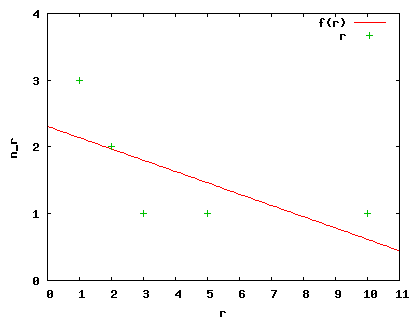
\includegraphics[scale=0.55]{figures/fit.png}
\column{.3\textwidth}
{\small
\begin{eqnarray*}
f(r) & = & a + b * r \\
a & = & 2.3 \\
b & = & -0.17 
\end{eqnarray*}
\begin{tabular}{ll}
\hline
$r$ & $n_r = f(r)$  \\
\hline
$1$ & 2.14 \\
$2$ & 1.97 \\
$3$ & 1.80 \\
$4$ & 1.63 \\
$5$ & 1.46 \\
$6$ & 1.29 \\
$7$ & 1.12 \\
$8$ & 0.95 \\
$9$ & 0.78 \\
$10$ & 0.61 \\
$11$ & 0.44 \\
\hline
\end{tabular}
}
\end{columns}
\end{frame}


\begin{frame}
\frametitle{Comparison between Add-one and Good-Turing}
\centering
\begin{tabular}{lllll}
\hline
freq & num with freq $r$ & NS    & Add1  & SGT   \\
$r$  & $n_r$ & $p_r$ & $p_r$ & $p_r$ \\
\hline
0  &  0 & 0    & 0.0294 & 0.12 \\
1  &  3 & 0.04 & 0.0588 & 0.03079 \\
2  &  2 & 0.08 & 0.0882 & 0.06719 \\
3  &  1 & 0.12 & 0.1176 & 0.1045 \\
5  &  1 & 0.2  & 0.1764 & 0.1797 \\
10 &  1 & 0.4  & 0.3235 & 0.3691 \\
\hline
\end{tabular}
\begin{itemize}[<+->]
\item $N = (1*3) + (2*2) + 3 + 5 + 10 = 25$
\item $V = 1 + 3 + 2 + 1 + 1 + 1 = 9$
\item Important: we added a new word type for unseen words. Let's call it UNK, the unknown word.
\item Check that: $1.0 == \sum_r n_r \times p_r$ \\
{\small $0.12 + (3 * 0.03079) + (2 * 0.06719) + 0.1045  + 0.1797 + 0.3691 = 1.0$ }
\end{itemize}
\end{frame}

\begin{frame}
\frametitle{Comparison between Add-one and Good-Turing}
\centering
\begin{tabular}{lllll}
\hline
freq & num with freq $r$ & NS    & Add1  & SGT   \\
$r$  & $n_r$ & $p_r$ & $p_r$ & $p_r$ \\
\hline
0  &  0 & 0    & 0.0294 & 0.12 \\
1  &  3 & 0.04 & 0.0588 & 0.03079 \\
2  &  2 & 0.08 & 0.0882 & 0.06719 \\
3  &  1 & 0.12 & 0.1176 & 0.1045 \\
5  &  1 & 0.2  & 0.1764 & 0.1797 \\
10 &  1 & 0.4  & 0.3235 & 0.3691 \\
\hline
\end{tabular}
\begin{itemize}[<+->]
\item NS = No smoothing: $p_r = \frac{r}{N}$
%%$(3 * 0.04) + (2 * 0.08) + 0.12 + 0.2 + 0.4 = 1.0$
\item Add1 = Add-one smoothing: $p_r = \frac{1 + r}{V + N}$
%%$0.0294 + (3 * 0.0588) + (2* 0.0882) + 0.1176 + 0.1764 + 0.3235 = 1.0$
\item SGT = Simple Good-Turing: $p_0 = \frac{n_1}{N}$, $p_r = \frac{(r+1) \frac{n_{r+1}}{n_r}}{N}$ \\
with linear interpolation for missing values where $n_{r+1} = 0$ \\
{\small (Gale and Sampson, 1995) \textit{http://www.grsampson.net/AGtf1.html}}
%%$0.12 + (3 * 0.03079) + (2 * 0.06719) + 0.1045  + 0.1797 + 0.3691 = 1.0$
\end{itemize}
\end{frame}

\subsection{Smoothing by Interpolation}

\begin{frame}
\frametitle{Using unigrams to smooth bigrams: incorrect version}
\[ P(w_i~\mid~w_{i-1}) = \frac{ c(w_{i-1},w_i) } { c(w_{i-1}) } \]
\begin{itemize}[<+->]
\item In add-one or Good-Turing: $P(\textsf{the}~\mid~\textsf{string}) = P(\textsf{Fonz}~\mid~\textsf{string})$
\item If $c(w_{i-1},w_i) = 0$, then use $P(w_i)$ (back off)
\item Works for trigrams too: back off to bigrams and then unigrams
\item Problem: probabilities get mixed up (unseen bigrams, for example will get higher probabilities than seen bigrams)
\end{itemize}
\end{frame}
\end{comment}

\subsection{Interpolation: Jelinek-Mercer Smoothing}

\begin{frame}
\frametitle{Interpolation: Jelinek-Mercer Smoothing}
\[ P_{ML}(w_i~\mid~w_{i-1}) = \frac{ c(w_{i-1},w_i) } { c(w_{i-1}) } \]
\begin{itemize}[<+->]
\item $P_{JM}(w_i~\mid~w_{i-1}) = {\color{blue} \lambda} P_{ML}(w_i~\mid~w_{i-1}) +  {\color{blue} (1 - \lambda) }P_{ML}(w_{i})$ \\
 where, $0 \leq \lambda \leq 1$
\item Jelinek and Mercer (1980) describe an elegant form of this {\bf interpolation}:
\[ P_{JM}(\textsf{$n$gram}) = \lambda P_{ML}(\textsf{$n$gram}) + (1 - \lambda) P_{JM}(\textsf{$n-1$gram}) \]
\item What about $P_{JM}(w_i)$? \\
For missing unigrams: $P_{JM}(w_i) = \lambda P_{ML}(w_i) + (1 - \lambda) \frac{\delta}{V}$ \\
$0 < \delta \leq 1$
\end{itemize}
\end{frame}

\begin{frame}
\frametitle{Interpolation: Finding $\lambda$}
\[ P_{JM}(\textsf{$n$gram}) = \lambda P_{ML}(\textsf{$n$gram}) + (1 - \lambda) P_{JM}(\textsf{$n-1$gram}) \]
\begin{itemize}[<+->]
\item Deleted Interpolation (Jelinek, Mercer) \\
compute $\lambda$ values to minimize cross-entropy on {\bf held-out} data which is \alert{deleted} from the initial set of training data
\item Improved JM smoothing, a separate $\lambda$ for each $w_{i-1}$: 
\[ P_{JM}(w_i \mid w_{i-1}) = {\color{blue} \lambda(w_{i-1})} P_{ML}(w_i \mid w_{i-1}) + {\color{blue} (1 - \lambda(w_{i-1}))} P_{ML}(w_i) \]
\end{itemize}
\end{frame}

\subsection{Backoff Smoothing with Discounting}

\begin{comment}
\subsubsection{Katz Backoff}
\begin{frame}
\frametitle{Backoff Smoothing: Katz Backoff}
\begin{itemize}[<+->]
\item Use smoothing over counts for backoff smoothing.
\item Also called discounting since we remove some probability from observed events.
\item Katz Backoff (include Good-Turing with Backoff Smoothing)
\[ P_{\textit{katz}}(y~\mid~x) = \left\{ 
\begin{array}{cc}
\frac{ c^\ast(xy) }{ c(x) } & \textsf{ if $c(xy) > 0$} \\
\alpha(x) P_{\textit{katz}} (y) & \textsf{otherwise}
\end{array}
\right. \]
\end{itemize}
\end{frame}
\end{comment}

\begin{frame}
\frametitle{Backoff Smoothing with Discounting}
\begin{itemize}[<+->]
\item Absolute Discounting (aka \textit{abs}) (Ney, Essen, Kneser)
\[ P_{\textit{abs}}(y~\mid~x) = \left\{ 
\begin{array}{cc}
\frac{ c(xy) - D }{ c(x) } & \textsf{ if $c(xy) > 0$} \\
\alpha(x) P(y) & \textsf{otherwise}
\end{array}
\right. \]
\item where $\alpha(x)$ is chosen to make sure that $P_{\textit{abs}}(y~\mid~x)$ is a proper probability
\[ \alpha(x) = 1 - \sum_y \frac{ c(xy) - D }{ c(x) } \]
\end{itemize}
\end{frame}

\begin{frame}
\frametitle{Backoff Smoothing with Discounting}
\begin{center}
\begin{tabular}{ | l | l | l | l | }
\hline
$x$ & $c(x)$ & $c(x)-D$ & $\frac{c(x)-D}{c(\textit{the})}$ \\
\hline
the & 48 & & \\
the,dog & 15 & 14.5 & 14.5/48 \\
the,woman & 11 & 10.5 & 10.4/48 \\
the,man & 10 & 9.5 & 9.5/48 \\
the,park & 5 & 4.5 & 4.5/48 \\
the,job & 2 & 1.5 & 1.5/48 \\
the,telescope & 1 & 0.5 & 0.5/48 \\
the,manual & 1 & 0.5 & 0.5/48 \\
the,afternoon & 1 & 0.5 & 0.5/48 \\
the,country & 1 & 0.5 & 0.5/48 \\
the,street & 1 & 0.5 & 0.5/48 \\
\hline
TOTAL & & & 0.8958 \\
\hline
the,UNK & 0 & & 0.1042 \\
\hline
\end{tabular}
\end{center}
\end{frame}


\begin{comment}
\begin{frame}
\frametitle{Backoff Smoothing with Discounting}
\begin{itemize}[<+->]
\item Kneser-Ney smoothing \\
$P(\textsf{Francisco}~\mid~\textsf{eggplant}) > P(\textsf{stew}~\mid~\textsf{eggplant})$
\begin{itemize}[<+->]
\item {\em Francisco} is common, so interpolation gives $P(\textsf{Francisco}~\mid~\textsf{eggplant})$ a high value
\item But {\em Francisco} occurs in few contexts (only after {\em San})
\item {\em stew} is common, {\bf and} occurs in many contexts
\item Hence weight the interpolation based on number of contexts for the word using discounting
\end{itemize}
\end{itemize}
\end{frame}

\end{comment}

\lecture{Evaluating Language Models}{}
\section{Evaluating Language Models}
\frame{\tableofcontents[currentsection]}

\begin{frame}
\frametitle{Evaluating Language Models}
\begin{itemize}[<+->]
\item So far we've seen the probability of a sentence: $P(w_0, \ldots, w_n)$
\item What is the probability of a collection of sentences, that is what is the probability of an unseen test corpus $T$
\item Let $T = s_0, \ldots, s_m$ be a test corpus with sentences $s_i$
\item $T$ is assumed to be separate from the training data used to train our language model $P(s)$
\item What is $P(T)$?
\end{itemize}
\end{frame}

\begin{frame}
\frametitle{Evaluating Language Models: Independence assumption}
\begin{itemize}[<+->]
\item $T = s_0, \ldots, s_m$ is the text corpus with sentences $s_0$ through $s_m$
\item $P(T) = P(s_0, s_1, s_2, \ldots, s_m)$ -- but each sentence is independent from the other sentences
\item $P(T) = P(s_0) \cdot P(s_1) \cdot P(s_2) \cdot \ldots \cdot P(s_m) = \prod_{i=0}^m P(s_i)$ 
\item $P(s_i) = P(w_0^{(i)}, \ldots, w_{n_i}^{(i)})$ -- which can be any $n$-gram language model
\item A language model is better if the value of $P(T)$ is higher for unseen sentences $T$, we want to maximize:
\[ P(T) = \prod_{i=0}^m P(s_i) \]
\end{itemize}
\end{frame}

\begin{frame}
\frametitle{Evaluating Language Models: Computing the Average}
\begin{itemize}[<+->]
\item However, $T$ can be any arbitrary size
\item $P(T)$ will be lower if $T$ is larger.
\item Instead of the probability for a given $T$ we can compute the {\em average} probability.
\item $M$ is the total number of tokens in the test corpus $T$:
\[ M = \sum_{i=0}^m \textsf{length}(s_i) \]
\item The average {\em log} probability of the test corpus $T$ is:
\[ \frac{1}{M} \log_2 \prod_{i=0}^m P(s_i) = \frac{1}{M} \sum_{i=0}^m \log_2 P(s_i) \]
\end{itemize}
\end{frame}

\begin{frame}
\frametitle{Evaluating Language Models: Perplexity}
\begin{itemize}[<+->]
\item The average {\em log} probability of the test corpus $T$ is:
\[ \ell = \frac{1}{M} \sum_{i=0}^m \log_2 P(s_i) \]
\item Note that $\ell$ is a negative number
\item We evaluate a language model using {\em Perplexity} which is $2^{-\ell}$
\end{itemize}
\end{frame}

\begin{frame}
\frametitle{Evaluating Language Models}
\begin{alertblock}{Question}
Show that:
\[ 2^{- \frac{1}{M} \log_2 \prod_{i=0}^m P(s_i)} = \frac{1}{\sqrt[M]{\prod_{i=0}^m P(s_i)}} \]
\end{alertblock}
\end{frame}

\begin{frame}
\frametitle{Evaluating Language Models}
\begin{alertblock}{Question}
What happens to $2^{- \ell}$ if any $n$-gram probability for computing $P(T)$ is zero?
\end{alertblock}
\end{frame}

\begin{frame}
\frametitle{Evaluating Language Models: Typical Perplexity Values}
\begin{block}{From 'A Bit of Progress in Language Modeling' by Chen and Goodman}
\centering
\begin{tabular}{ll}
Model & Perplexity \\
\hline
unigram & 955 \\
bigram & 137 \\
trigram & 74 
\end{tabular}
\end{block}
\end{frame}

\begin{frame}
\frametitle{Evaluating Language Models: Typical Perplexity Values}
\begin{block}{{\small From 'One Billion Word Benchmark for Measuring Progress in Statistical Language Modeling' by Chelba+ (Google)}}
\centering
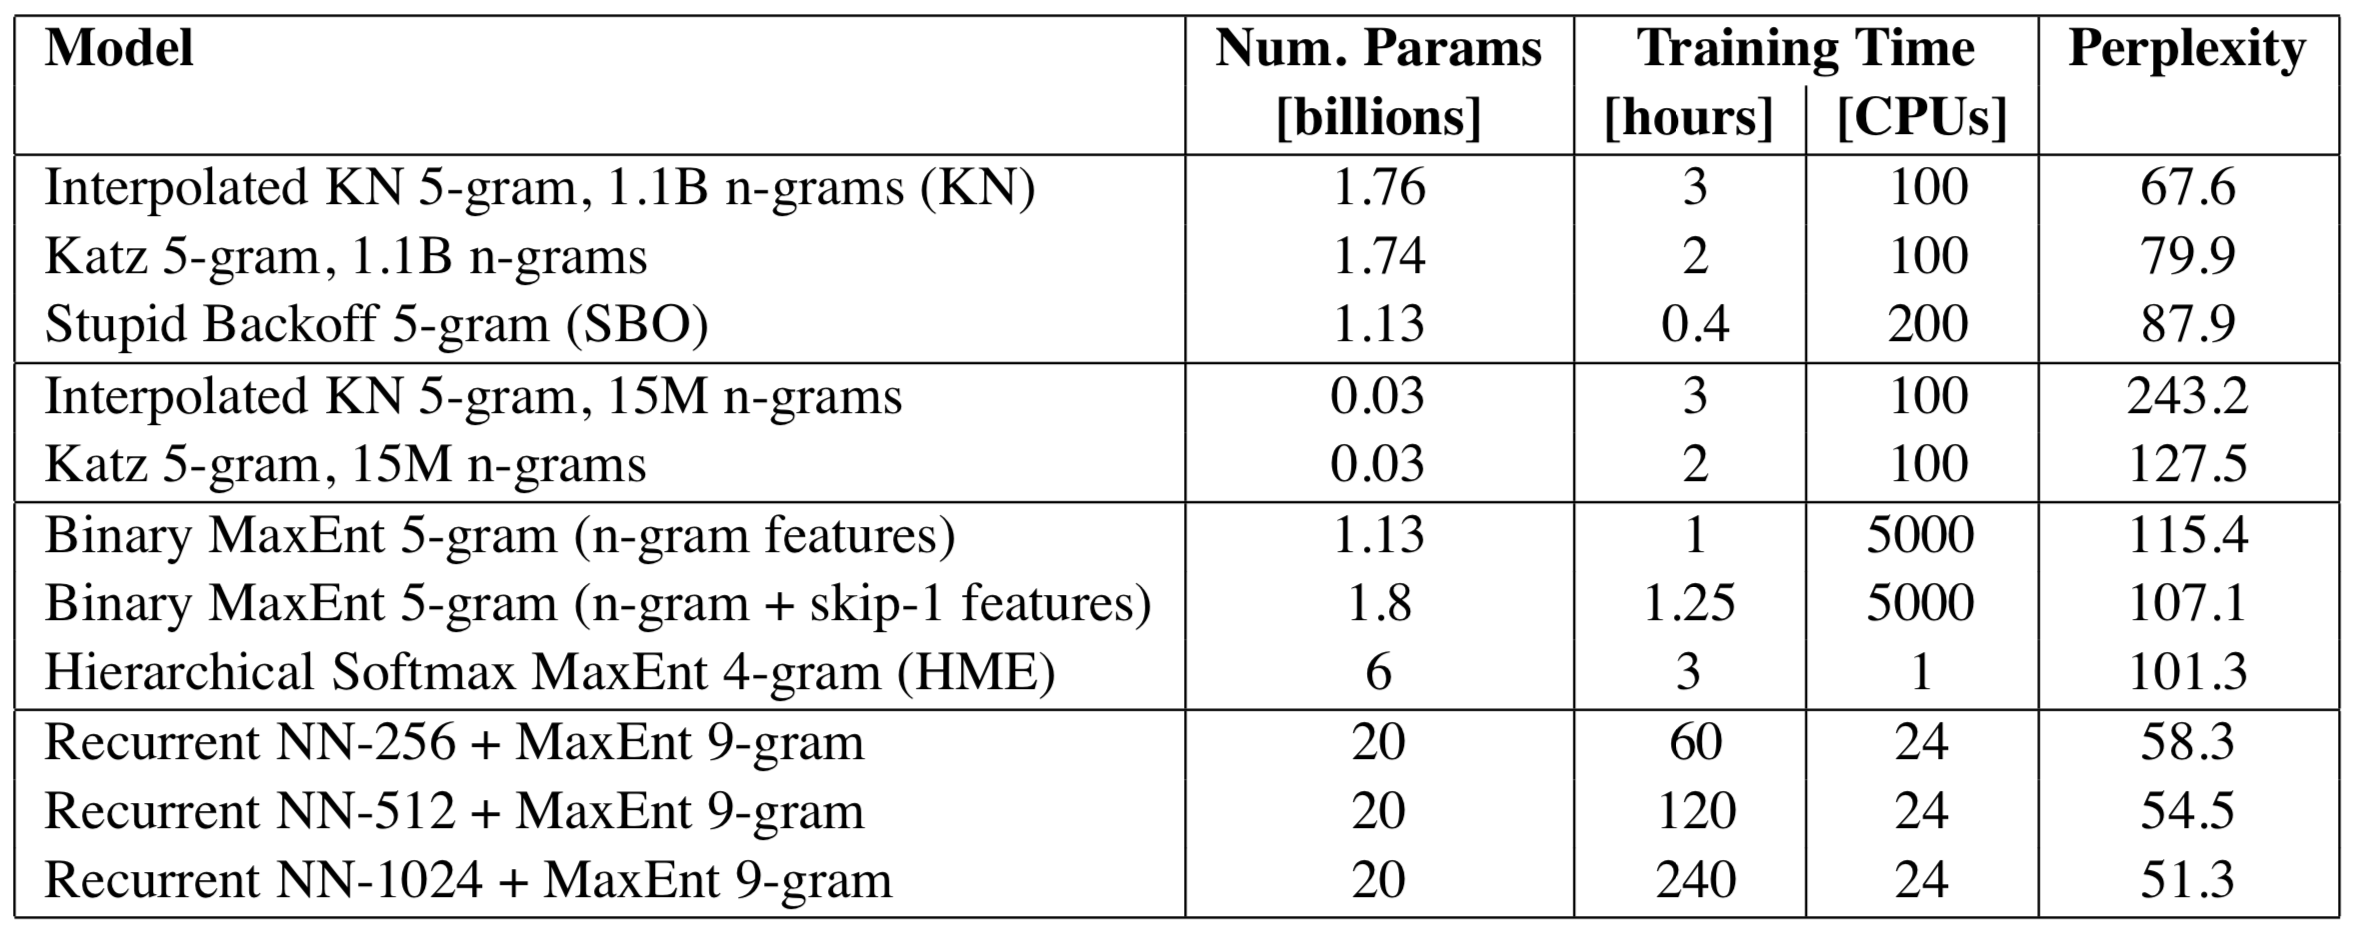
\includegraphics[scale=.25]{figures/1b-benchmark-test.png}
\end{block}
\end{frame}

\lecture{Event space in Language Models}{}
\section{Event Space for $n$-gram Models}

\begin{frame}
\frametitle{Trigram Models}
\begin{itemize}[<+->]
\item The trigram model:\\
$P(w_1, w_2, \ldots, w_n) = P(w_1) \times P(w_2~\mid~w_1) \times 
P(w_3~\mid~w_1, w_2) \times P(w_4~\mid~w_2, w_3) 
\times \ldots P(w_i~\mid~w_{i-2}, w_{i-1}) \ldots 
\times P(w_n~\mid~w_{n-2}, \ldots, w_{n-1}) $
\item Notice that the length of the sentence $n$ is variable
\item What is the event space?
\end{itemize}
\end{frame}

\newcommand{\lmstop}{\mbox{\texttt stop}}

\begin{frame}
\frametitle{The {\tt stop} symbol}
\begin{itemize}[<+->]
\item Let ${\cal V} = \{ a, b \}$ and the language $L$ be ${\cal V}^\ast$
\item Consider a unigram model: $P(a) = P(b) = 0.5$
\item So strings in this language $L$ are:
\begin{eqnarray*}
a\ \lmstop & 0.5 \\
b\ \lmstop & 0.5 \\
aa\ \lmstop & 0.5^2 \\
bb\ \lmstop & 0.5^2 \\
\vdots
\end{eqnarray*}
\item The sum over all strings in $L$ should be equal to 1:
\[ \sum_{w \in L} P(w) = 1 \]
\item But $P(a) + P(b) + P(aa) + P(bb) = 1.5$ !! 
\end{itemize}
\end{frame}

\begin{frame}
\frametitle{The {\tt stop} symbol}
\begin{itemize}[<+->]
\item What went wrong? \\
We need to model variable length sequences
\item Add an explicit probability for the \lmstop symbol: 
\[ P(a) = P(b) = 0.25  \]
\[ P(\lmstop) = 0.5 \]
\item $P(\lmstop) = 0.5$, $P(a\ \lmstop) = P(b\ \lmstop) = 0.25 \times 0.5 = 0.125$, 
$P(aa\ \lmstop) = 0.25^2 \times 0.5 = 0.03125$ (now the sum is no longer greater than one)
\end{itemize}
\end{frame}

\begin{frame}
\frametitle{The {\tt stop} symbol}
\begin{itemize}[<+->]
\item With this new {\tt stop} symbol we can show that $\sum_w P(w) = 1$ \\
Notice that the probability of any sequence of length $n$ is $0.25^n \times 0.5$ \\
Also there are $2^n$ sequences of length $n$
\end{itemize}
\begin{eqnarray}
\lefteqn{\sum_w P(w) = } \nonumber \\
&& \sum_{n=0}^{\infty} 2^n \times 0.25^n \times 0.5 \nonumber \\
&& \sum_{n=0}^{\infty} 0.5^n \times 0.5 = \sum_{n=0}^{\infty} 0.5^{n+1} \nonumber \\
&& \sum_{n=1}^{\infty} 0.5^n = 1 \nonumber
\end{eqnarray}
\end{frame}

\begin{frame}
\frametitle{The {\tt stop} symbol}
\begin{itemize}[<+->]
\item With this new {\tt stop} symbol we can show that $\sum_w P(w) = 1$ \\
Using $p_s = P(\texttt{stop})$ the probability of any sequence of length $n$ is $p(n) = p(w_1, \ldots, w_{n-1}) \times p_s(w_n)$ \\
\end{itemize}
\begin{eqnarray*}
\sum_w P(w) &=& \sum_{n=0}^{\infty} p(n) \sum_{w_1, \ldots, w_n} p(w_1, \ldots, w_n) \\
&=& \sum_{n=0}^{\infty} p(n) \sum_{w_1, \ldots, w_n} \prod_{i=0}^n p(w_i)
\end{eqnarray*}
\begin{eqnarray*}
\lefteqn{\sum_{w_1, \ldots, w_n} \prod_i p(w_i) = } \\
&& \sum_{w_1} \sum_{w_2} \ldots \sum_{w_n} p(w_1) p(w_2) \ldots p(w_n) = 1
\end{eqnarray*}
\end{frame}

\begin{frame}
\frametitle{The {\tt stop} symbol}
\begin{eqnarray*}
\sum_{w_1} \sum_{w_2} \ldots \sum_{w_n} p(w_1) p(w_2) \ldots p(w_n) &=& 1
\end{eqnarray*}
\begin{eqnarray*}
\sum_{n=0}^\infty p(n) &=& \sum_{n=0}^\infty p_s(1 - p_s)^n \\
&=& p_s \sum_{n=0}^\infty (1 - p_s)^n \\
&=& p_s \frac{1}{1-(1-p_s)} = p_s \frac{1}{p_s} = 1
\end{eqnarray*}
\end{frame}


\section*{Acknowledgements}

\begin{frame}
\centering
\begin{alertblock}{Acknowledgements}
Many slides borrowed or inspired from lecture notes by Michael Collins, Chris Dyer, Kevin Knight, Philipp Koehn, Adam Lopez, Graham Neubig and Luke Zettlemoyer from their NLP course materials. 

\bigskip

All mistakes are my own.

\bigskip

A big thank you to all the students who read through these notes and helped me improve them.

\end{alertblock}
\end{frame}



\end{document}
 
